\documentclass[11pt,a4paper]{article}

\usepackage{amsmath,amssymb,graphicx,geometry,hyperref,listings,xcolor}
\usepackage[utf8]{inputenc}
\usepackage[T1]{fontenc}
\usepackage{booktabs,array,tabularx,enumitem,multirow,colortbl,parskip}
\usepackage{tikz,pgfplots}
\pgfplotsset{compat=1.18}
\usetikzlibrary{arrows.meta,shapes.geometric,positioning,
                decorations.pathreplacing,calc,backgrounds}
\usepackage{tcolorbox}
\tcbuselibrary{skins}

\geometry{margin=2.5cm}
\renewcommand{\arraystretch}{1}
\title{Options \& Commodity Derivatives Analytics Platform}
\author{Adam El Gbouri}
\date{May 2026}
\renewcommand{\arraystretch}{1}
\renewcommand{\arraystretch}{1.45}

\definecolor{amber}{RGB}{240,165,0}
\definecolor{accentblue}{RGB}{31,111,235}
\definecolor{lightgray}{RGB}{246,248,250}
\definecolor{darktext}{RGB}{26,26,46}
\definecolor{signalgreen}{RGB}{26,127,55}
\definecolor{signalred}{RGB}{207,34,46}
\definecolor{signalgray}{RGB}{110,118,129}
\definecolor{boxbg}{RGB}{237,244,255}
\definecolor{notebg}{RGB}{255,251,235}
\definecolor{noteborder}{RGB}{240,165,0}
\definecolor{purple}{RGB}{130,80,255}

\lstset{language=Python,basicstyle=\ttfamily\small,
  keywordstyle=\color{accentblue},commentstyle=\color{signalgray},
  stringstyle=\color{amber},breaklines=true,
  backgroundcolor=\color{lightgray},frame=single,framerule=0.4pt,
  rulecolor=\color{signalgray},xleftmargin=8pt,xrightmargin=8pt}

\newenvironment{keybox}[1]{%
  \begin{tcolorbox}[colback=boxbg,colframe=accentblue,
    fonttitle=\bfseries\small,title=#1,
    left=8pt,right=8pt,top=6pt,bottom=6pt,boxrule=0.5pt]}
{\end{tcolorbox}}

\newenvironment{notebox}{%
  \begin{tcolorbox}[colback=notebg,colframe=noteborder,
    left=8pt,right=8pt,top=5pt,bottom=5pt,boxrule=0.5pt]}
{\end{tcolorbox}}

\pgfplotsset{
  every axis title/.style={at={(0.5,1.05)},anchor=south,
    font=\small\bfseries,color=darktext},
  every axis legend/.style={fill=white,draw=signalgray!50,
    font=\small,cells={anchor=west},inner sep=4pt},
  grid style={draw=gray!18,line width=0.3pt},
  tick label style={font=\footnotesize},
  label style={font=\small},
}

\begin{document}

\maketitle

%==============================================================================
\section{Introduction}
%==============================================================================

\subsection{What is a Commodity Derivative?}

A commodity derivative is a financial contract whose payoff depends on the
future price of a raw material: crude oil, natural gas, gold, corn, and so on.
Unlike equity derivatives, commodity derivatives are almost universally priced on
\textbf{futures prices}, not spot prices, because:

\begin{itemize}[itemsep=3pt]
\item Futures are liquid, transparent and observable at every maturity on organised exchanges.
\item The futures price already embeds storage costs, financing and convenience yield. No additional cost-of-carry adjustment is needed in the pricing model.
\item Physical delivery is impractical for most market participants; futures allow pure price exposure without storage obligations.
\end{itemize}

Three types of participants use commodity derivatives:

\medskip
\begin{center}
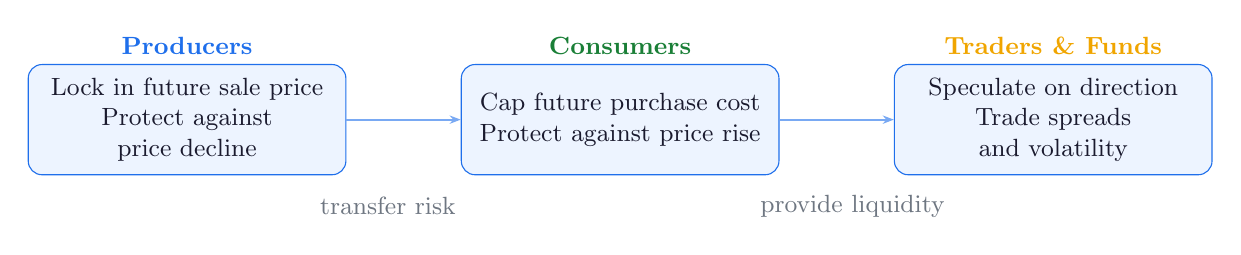
\begin{tikzpicture}[
  box/.style={draw=accentblue,fill=boxbg,rounded corners=5pt,
              text width=3.8cm,minimum height=1.4cm,
              font=\small,align=center,text=darktext},
  arr/.style={-{Stealth[length=4pt]},thick,color=accentblue!60}]
\node[box,label={[font=\small\bfseries,color=accentblue]above:Producers}]
  (p) at (0,0)
  {Lock in future sale price\\Protect against price decline};
\node[box,label={[font=\small\bfseries,color=signalgreen]above:Consumers}]
  (c) at (5.5,0)
  {Cap future purchase cost\\Protect against price rise};
\node[box,label={[font=\small\bfseries,color=amber]above:Traders \& Funds}]
  (t) at (11,0)
  {Speculate on direction\\Trade spreads and volatility};
\draw[arr] (p.east)--(c.west);
\draw[arr] (c.east)--(t.west);
\node[font=\small,color=signalgray] at (2.55,-1.1) {transfer risk};
\node[font=\small,color=signalgray] at (8.45,-1.1) {provide liquidity};
\end{tikzpicture}
\end{center}

\subsection{Product Overview}

OCDAP implements six pricing engines covering the full spectrum of commodity
derivatives used by trading desks:

\medskip
\begin{center}
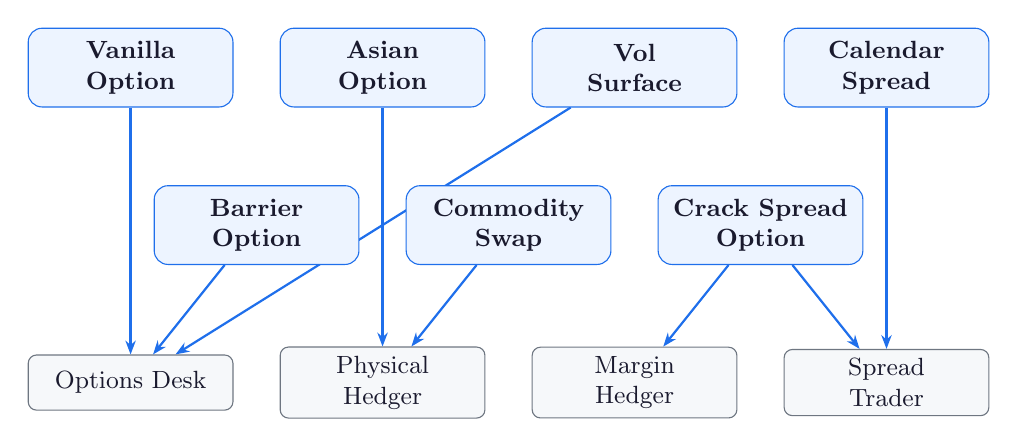
\begin{tikzpicture}[
  prod/.style={draw=accentblue,fill=boxbg,rounded corners=5pt,
               minimum width=2.6cm,minimum height=1.0cm,
               font=\small\bfseries,text=darktext,align=center},
  user/.style={draw=signalgray,fill=lightgray,rounded corners=3pt,
               minimum width=2.6cm,minimum height=0.7cm,
               font=\small,text=darktext,align=center},
  arrow/.style={-{Stealth[length=5pt]},thick,color=accentblue}]
\node[prod](v)   at (0,0)      {Vanilla\\Option};
\node[prod](a)   at (3.2,0)    {Asian\\Option};
\node[prod](vs)  at (6.4,0)    {Vol\\Surface};
\node[prod](cal) at (9.6,0)    {Calendar\\Spread};
\node[prod](s)   at (4.8,-2.0) {Commodity\\Swap};
\node[prod](b)   at (1.6,-2.0) {Barrier\\Option};
\node[prod](c)   at (8.0,-2.0) {Crack Spread\\Option};
\node[user](u1) at (0,-4)      {Options Desk};
\node[user](u2) at (3.2,-4)    {Physical\\Hedger};
\node[user](u3) at (6.4,-4)    {Margin\\Hedger};
\node[user](u4) at (9.6,-4)    {Spread\\Trader};
\draw[arrow](v)--(u1);
\draw[arrow](a)--(u2);
\draw[arrow](c)--(u3); \draw[arrow](c)--(u4);
\draw[arrow](cal)--(u4);
\draw[arrow](s)--(u2);
\draw[arrow](b)--(u1);
\begin{pgfonlayer}{background}
  \draw[arrow](vs)--(u1);
\end{pgfonlayer}
\end{tikzpicture}
\end{center}

\medskip
\begin{center}
\renewcommand{\arraystretch}{1.5}
\begin{tabularx}{\textwidth}{>{\bfseries}l X l}
\toprule
Tab & Product & Model \\
\midrule
Vanilla Options   & European call/put on futures                              & Black-76 \\
Asian Options     & Arithmetic/geometric average-price option                 & MC + Kemna-Vorst \\
Crack Spread      & Option on refining margin $F_2-F_1$                       & Kirk (1995) \\
Calendar Spread   & Option on curve slope $F_\text{near}-F_\text{far}$        & Kirk on term structure \\
Commodity Swaps   & Fixed-for-floating commodity swap                         & Discounted cashflows \\
Barrier Options   & Knock-in / knock-out (daily monitoring)                   & Daily Monte Carlo \\
Vol Surface       & Parametric implied volatility surface                     & Black-76 + skew \\
Forward Curve     & Live futures curve + cost-of-carry extension              & Yahoo / TradingView \\
\bottomrule
\end{tabularx}
\end{center}

%==============================================================================
\section{Architecture}
%==============================================================================

\subsection{The Pricing Pipeline}

Every product in OCDAP follows the same five-step pipeline:

\medskip
\begin{center}
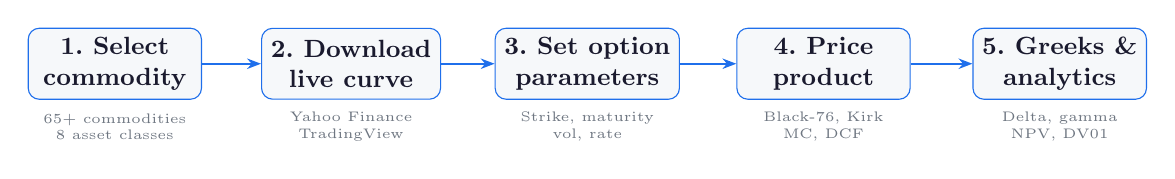
\begin{tikzpicture}[
  box/.style={draw=accentblue,fill=lightgray,rounded corners=4pt,
              minimum width=2.2cm,minimum height=0.9cm,
              font=\small\bfseries,text=darktext,align=center},
  arr/.style={-{Stealth[length=5pt]},thick,color=accentblue}]
\node[box](A) at (0,0)    {1.~Select\\commodity};
\node[box](B) at (3.0,0)  {2.~Download\\live curve};
\node[box](C) at (6.0,0)  {3.~Set option\\parameters};
\node[box](D) at (9.0,0)  {4.~Price\\product};
\node[box](E) at (12.0,0) {5.~Greeks \&\\analytics};
\draw[arr](A)--(B); \draw[arr](B)--(C);
\draw[arr](C)--(D); \draw[arr](D)--(E);
% Step labels below
\node[font=\tiny,color=signalgray,align=center] at (0,-0.8)
  {65+ commodities\\8 asset classes};
\node[font=\tiny,color=signalgray,align=center] at (3.0,-0.8)
  {Yahoo Finance\\TradingView};
\node[font=\tiny,color=signalgray,align=center] at (6.0,-0.8)
  {Strike, maturity\\vol, rate};
\node[font=\tiny,color=signalgray,align=center] at (9.0,-0.8)
  {Black-76, Kirk\\MC, DCF};
\node[font=\tiny,color=signalgray,align=center] at (12.0,-0.8)
  {Delta, gamma\\NPV, DV01};
\end{tikzpicture}
\end{center}

\subsection{Expiry-Aware Ticker Generation}

A critical design choice: OCDAP always downloads the \textbf{true front month},
not an expired contract. Standard futures expire approximately on the 20th of
the month before delivery.

\medskip
\begin{center}
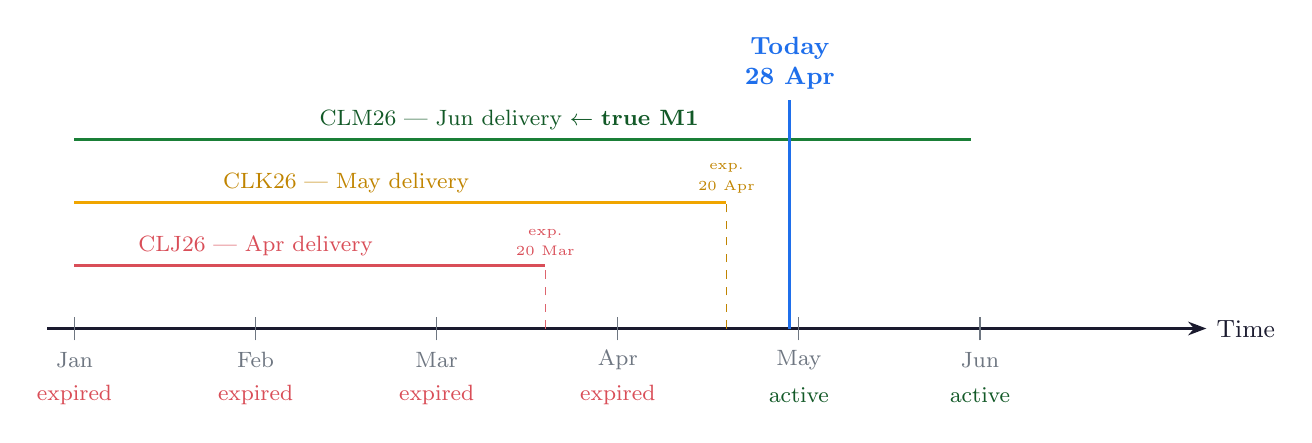
\begin{tikzpicture}[xscale=1.15]
\draw[-{Stealth},thick,color=darktext](-0.3,0)--(12.5,0)
  node[right,font=\small]{Time};
\foreach \x/\l in {0/Jan,2/Feb,4/Mar,6/Apr,8/May,10/Jun}{
  \draw[thin,color=signalgray](\x,-0.15)--(\x,0.15);
  \node[font=\footnotesize,color=signalgray]at(\x,-0.4){\l};}
\draw[very thick,color=signalred!80]  (0,0.8)--(5.2,0.8);
\draw[very thick,color=amber]         (0,1.6)--(7.2,1.6);
\draw[very thick,color=signalgreen]   (0,2.4)--(9.9,2.4);
\node[font=\footnotesize,color=signalred!80]  at(2.0,1.05) {CLJ26 --- Apr delivery};
\node[font=\footnotesize,color=amber!80!black]at(3.0,1.85) {CLK26 --- May delivery};
\node[font=\footnotesize,color=signalgreen!70!black]at(4.8,2.65)
  {CLM26 --- Jun delivery\ $\leftarrow$ \textbf{true M1}};
\draw[dashed,thin,color=signalred!70](5.2,0)--(5.2,0.8)
  node[above,font=\tiny,color=signalred!80]{\shortstack{exp.\\20 Mar}};
\draw[dashed,thin,color=amber!80!black](7.2,0)--(7.2,1.6)
  node[above,font=\tiny,color=amber!80!black]{\shortstack{exp.\\20 Apr}};
\draw[very thick,color=accentblue](7.9,0)--(7.9,2.9)
  node[above,font=\small\bfseries,color=accentblue]{\shortstack{Today\\28 Apr}};
\node[font=\footnotesize,color=signalred!80]at(0,-0.85){expired};
\node[font=\footnotesize,color=signalred!80]at(2,-0.85){expired};
\node[font=\footnotesize,color=signalred!80]at(4,-0.85){expired};
\node[font=\footnotesize,color=signalred!80]at(6,-0.85){expired};
\node[font=\footnotesize,color=signalgreen!70!black]at(8,-0.85){active};
\node[font=\footnotesize,color=signalgreen!70!black]at(10,-0.85){active};
\end{tikzpicture}
\end{center}

\medskip
Without this fix, Yahoo Finance returns stale prices from expired contracts:
on April 28 2026 it would return the last traded price of CLJ26 (expired March 20)
instead of the live price of CLM26 (the true front month).


%==============================================================================
\section{Black-76 Vanilla Option Pricer}
%==============================================================================

\subsection{Why Black-76 and Not Black-Scholes?}

\begin{center}
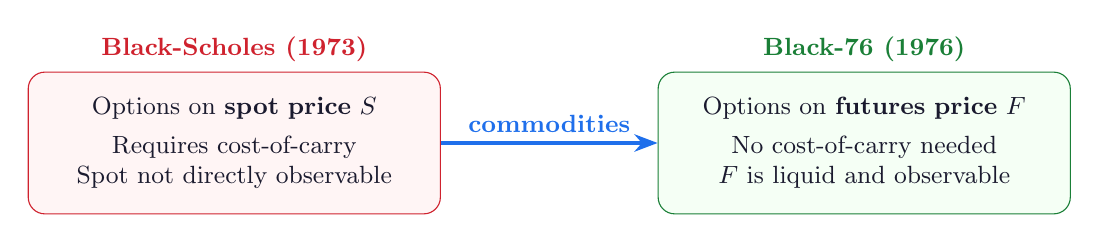
\begin{tikzpicture}
\node[draw=signalred,fill=red!4,rounded corners=6pt,
      text width=5.0cm,minimum height=1.8cm,
      font=\small,align=center,text=darktext,
      label={[font=\small\bfseries,color=signalred]above:Black-Scholes (1973)}]
  (bs) at (0,0)
  {Options on \textbf{spot price} $S$\\[3pt]
   Requires cost-of-carry\\
   Spot not directly observable};
\node[draw=signalgreen,fill=green!4,rounded corners=6pt,
      text width=5.0cm,minimum height=1.8cm,
      font=\small,align=center,text=darktext,
      label={[font=\small\bfseries,color=signalgreen]above:Black-76 (1976)}]
  (b76) at (8,0)
  {Options on \textbf{futures price} $F$\\[3pt]
   No cost-of-carry needed\\
   $F$ is liquid and observable};
\draw[-{Stealth},very thick,color=accentblue]
  (bs.east)--(b76.west)
  node[midway,above,font=\small\bfseries,color=accentblue]{commodities};
\end{tikzpicture}
\end{center}

The key insight: under the \textit{futures measure}, the futures price $F$ has zero drift. The discounting $e^{-rT}$ accounts for the fact that option premium is paid upfront but the futures payoff occurs at expiry.

\subsection{Pricing Formulas}

\begin{equation}
\boxed{C = e^{-rT}\bigl[F N(d_1)-K N(d_2)\bigr]}
\qquad
\boxed{P = e^{-rT}\bigl[K N(-d_2)-F N(-d_1)\bigr]}
\end{equation}
\begin{equation}
d_1=\frac{\ln(F/K)+\tfrac12\sigma^2 T}{\sigma\sqrt{T}},\qquad
d_2=d_1-\sigma\sqrt{T}
\end{equation}

\subsection{Payoff Diagrams}

\begin{center}
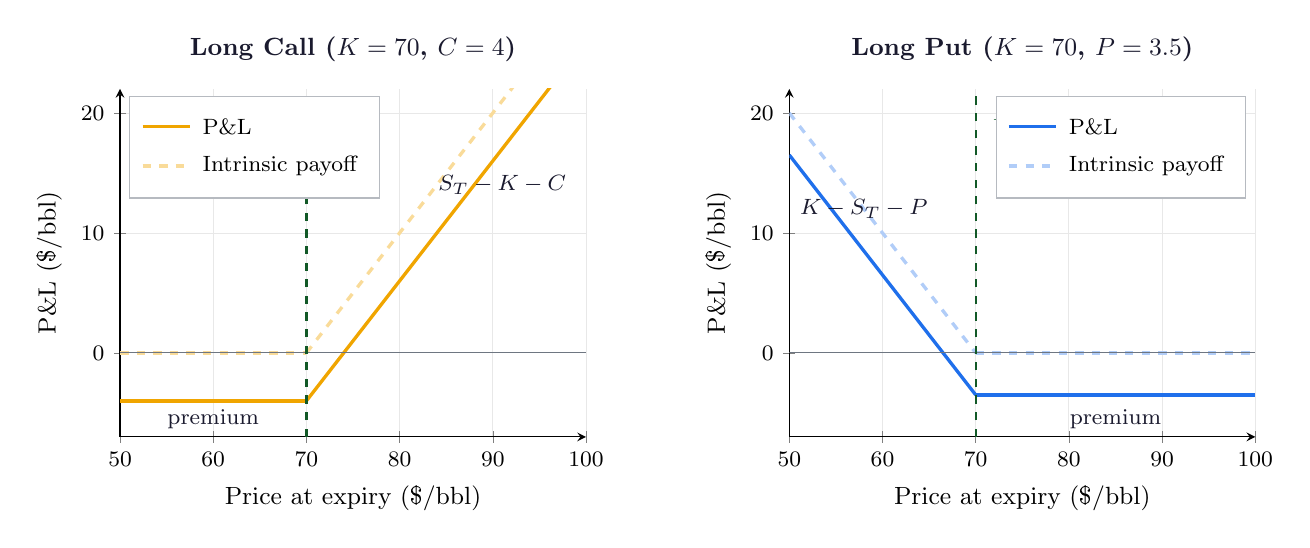
\begin{tikzpicture}
\begin{axis}[name=call,width=7.5cm,height=6cm,
  xlabel={Price at expiry (\$/bbl)},ylabel={P\&L (\$/bbl)},
  xmin=50,xmax=100,ymin=-7,ymax=22,
  grid=both,axis lines=left,
  title={Long Call ($K=70$, $C=4$)},
  legend style={at={(0.02,0.98)},anchor=north west,font=\footnotesize}]
\addplot[color=amber,very thick,domain=50:70]{-4};
\addplot[color=amber!40,very thick,dashed,domain=50:70]{0};
\addplot[color=amber!40,very thick,dashed,domain=70:100]{x-70};
\addplot[color=amber,very thick,domain=70:100]{x-74};
\addplot[color=signalgray,thin,domain=50:100]{0};
\draw[dashed,color=signalgreen!70!black,thick](axis cs:70,-7)--(axis cs:70,22);
\addlegendentry{P\&L}
\addlegendentry{Intrinsic payoff}
\node[font=\footnotesize,color=darktext]at(axis cs:60,-5.5){premium};
\node[font=\footnotesize,color=darktext]at(axis cs:91,14){$S_T-K-C$};
\node[font=\footnotesize,color=signalgreen!70!black]at(axis cs:73,20){$K$};
\end{axis}
\begin{axis}[at={(8.5cm,0)},width=7.5cm,height=6cm,
  xlabel={Price at expiry (\$/bbl)},ylabel={P\&L (\$/bbl)},
  xmin=50,xmax=100,ymin=-7,ymax=22,
  grid=both,axis lines=left,
  title={Long Put ($K=70$, $P=3.5$)},
  legend style={at={(0.98,0.98)},anchor=north east,font=\footnotesize}]
\addplot[color=accentblue,very thick,domain=50:70]{66.5-x};
\addplot[color=accentblue!35,very thick,dashed,domain=50:70]{70-x};
\addplot[color=accentblue!35,very thick,dashed,domain=70:100]{0};
\addplot[color=accentblue,very thick,domain=70:100]{-3.5};
\addplot[color=signalgray,thin,domain=50:100]{0};
\draw[dashed,color=signalgreen!70!black,thick](axis cs:70,-7)--(axis cs:70,22);
\addlegendentry{P\&L}
\addlegendentry{Intrinsic payoff}
\node[font=\footnotesize,color=darktext]at(axis cs:85,-5.5){premium};
\node[font=\footnotesize,color=darktext]at(axis cs:58,12){$K-S_T-P$};
\node[font=\footnotesize,color=signalgreen!70!black]at(axis cs:73,20){$K$};
\end{axis}
\end{tikzpicture}
\end{center}

\subsection{Greeks}

{\renewcommand{\arraystretch}{3.0}
\begin{center}
\begin{tabularx}{\textwidth}{c c X}
\toprule
\textbf{Greek} & \textbf{Formula (call)} & \textbf{Economic interpretation} \\
\midrule
$\Delta$ &
  $\displaystyle e^{-rT}N(d_1)$ &
  \textit{Delta}: number of futures needed to delta-hedge one option.
  ATM call $\approx 0.50$. Deep ITM $\to 1$, deep OTM $\to 0$. \\
$\Gamma$ &
  $\displaystyle\dfrac{e^{-rT}N'(d_1)}{F\sigma\sqrt{T}}$ &
  \textit{Gamma}: rate of change of delta per unit move in $F$.
  High $\Gamma$ means the hedge needs frequent and costly rebalancing. \\
$\mathcal{V}$ &
  $\displaystyle\dfrac{e^{-rT}F N'(d_1)\sqrt{T}}{100}$ &
  \textit{Vega}: P\&L per 1\% increase in implied vol.
  Long options have positive vega --- they gain when vol rises. \\
$\Theta$ &
  $\displaystyle\dfrac{-e^{-rT}F N'(d_1)\sigma}{2\sqrt{T}\cdot365}$ &
  \textit{Theta}: daily time decay. Always negative for long options.
  Largest near expiry when the option is at-the-money. \\
$\varrho$ &
  $\displaystyle\dfrac{-Te^{-rT}[FN(d_1)-KN(d_2)]}{100}$ &
  \textit{Rho}: P\&L per 1\% change in risk-free rate.
  Small for short-dated commodity options; much less important than vega. \\
\bottomrule
\end{tabularx}
\end{center}}

\subsection{Delta-Gamma Sensitivity Profile}

\begin{center}
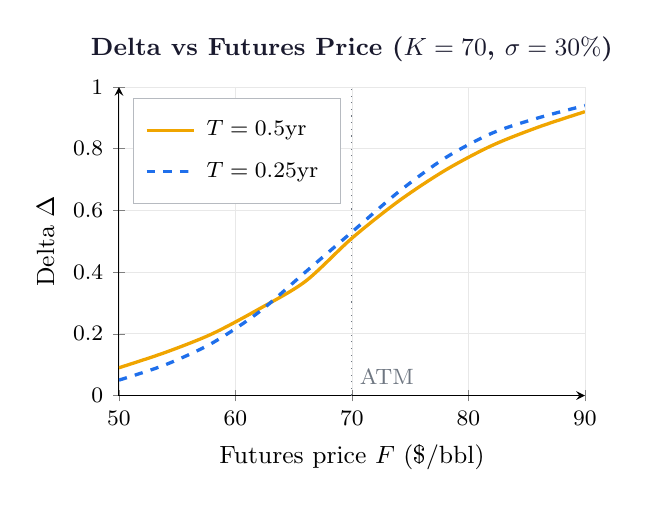
\begin{tikzpicture}
\begin{axis}[name=deltaplot,width=7.5cm,height=5.5cm,
  xlabel={Futures price $F$ (\$/bbl)},ylabel={Delta $\Delta$},
  xmin=50,xmax=90,ymin=0,ymax=1,
  grid=both,axis lines=left,
  title={Delta vs Futures Price ($K=70$, $\sigma=30\%$)},
  legend style={at={(0.031,0.965)},anchor=north west,font=\footnotesize}]
% Precomputed Black-76 delta at K=70, sigma=30%, r=4%
% T=0.5yr
\addplot[color=amber,very thick,smooth] coordinates {
  (50,0.09)(54,0.14)(58,0.20)(62,0.28)(66,0.37)
  (70,0.51)(74,0.63)(78,0.73)(82,0.81)(86,0.87)(90,0.92)};
% T=0.25yr
\addplot[color=accentblue,very thick,smooth,dashed] coordinates {
  (50,0.05)(54,0.10)(58,0.17)(62,0.27)(66,0.40)
  (70,0.53)(74,0.66)(78,0.77)(82,0.85)(86,0.90)(90,0.94)};
\addlegendentry{$T=0.5$yr}
\addlegendentry{$T=0.25$yr}
\draw[dotted,thin,color=signalgray](axis cs:70,0)--(axis cs:70,1);
\node[font=\footnotesize,color=signalgray]at(axis cs:73,0.06){ATM};
\end{axis}
\end{tikzpicture}
\hspace{0.5cm}
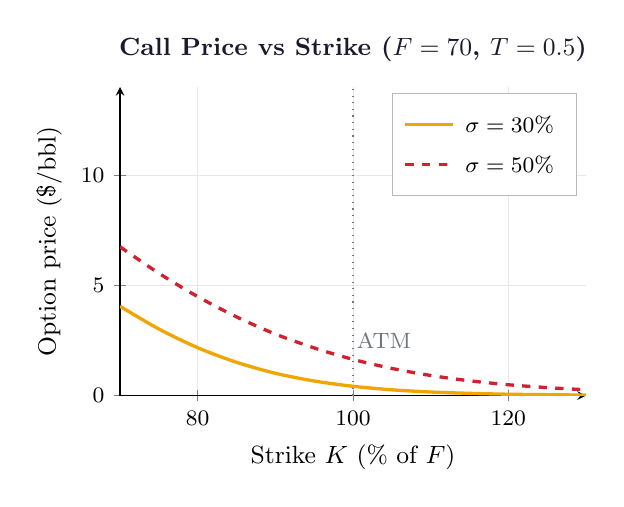
\begin{tikzpicture}
\begin{axis}[width=7.5cm,height=5.5cm,
  xlabel={Strike $K$ (\% of $F$)},ylabel={Option price (\$/bbl)},
  xmin=70,xmax=130,ymin=0,ymax=14,
  grid=both,axis lines=left,
  title={Call Price vs Strike ($F=70$, $T=0.5$)},
  legend style={at={(0.98,0.98)},anchor=north east,font=\footnotesize}]
% Precomputed Black-76 call prices, F=70, T=0.5, r=4%
% sigma=30%
\addplot[color=amber,very thick,smooth] coordinates {
  (70,4.05)(75,3.02)(80,2.17)(85,1.51)(90,1.01)(95,0.66)
  (100,0.42)(105,0.26)(110,0.16)(115,0.10)(120,0.06)(125,0.04)(130,0.02)};
% sigma=50%
\addplot[color=signalred,very thick,smooth,dashed] coordinates {
  (70,6.75)(75,5.55)(80,4.49)(85,3.57)(90,2.79)(95,2.16)
  (100,1.64)(105,1.23)(110,0.91)(115,0.67)(120,0.49)(125,0.36)(130,0.26)};
\addlegendentry{$\sigma=30\%$}
\addlegendentry{$\sigma=50\%$}
\draw[dotted,thin,color=signalgray](axis cs:100,0)--(axis cs:100,14);
\node[font=\footnotesize,color=signalgray]at(axis cs:104,2.5){ATM};
\end{axis}
\end{tikzpicture}
\end{center}

\subsection{Put-Call Parity}

\begin{equation}
C - P = e^{-rT}(F-K)
\end{equation}

OCDAP verifies this for every option pair. The residual is always below $10^{-4}$
and displayed as \texttt{\checkmark\ verified} in the dashboard.

%==============================================================================
\section{Asian Option Pricer}
%==============================================================================

\subsection{Why Asian Options in Commodity Markets?}

Asian options pay off on the \textbf{average price} over the option's life,
not the final price. This is the natural instrument for physical commodity
participants whose costs and revenues are priced on monthly averages.

\medskip
\begin{center}
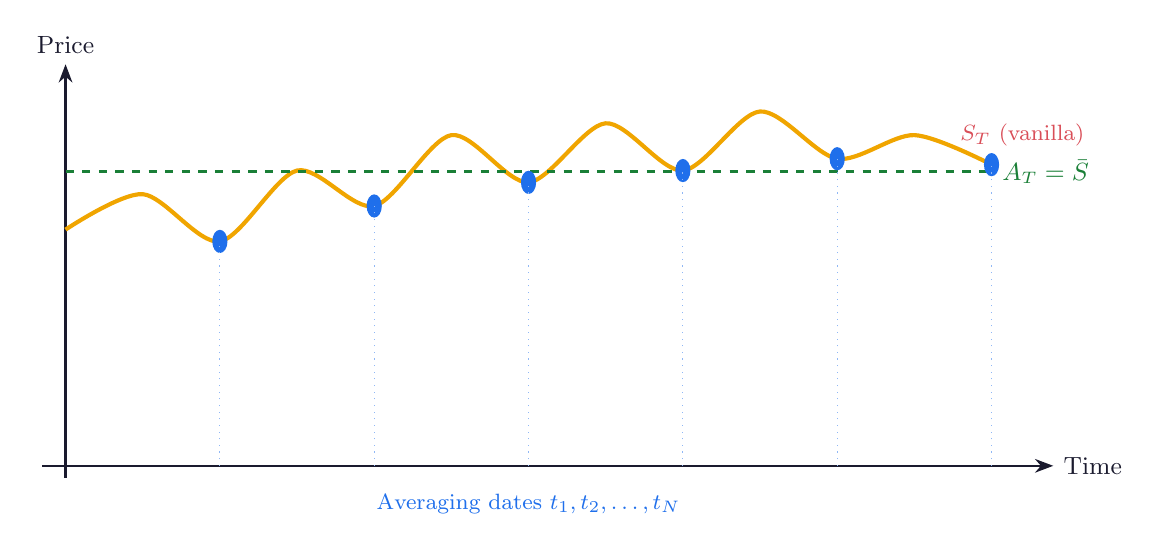
\begin{tikzpicture}[xscale=0.98,yscale=1.5]
\draw[-{Stealth},thick,color=darktext](-0.3,0)--(12.8,0)
  node[right,font=\small]{Time};
\draw[-{Stealth},thick,color=darktext](0,-0.1)--(0,3.4)
  node[above,font=\small]{Price};
\draw[color=amber,line width=1.5pt,smooth] plot coordinates
  {(0,2.0)(1,2.3)(2,1.9)(3,2.5)(4,2.2)(5,2.8)
   (6,2.4)(7,2.9)(8,2.5)(9,3.0)(10,2.6)(11,2.8)(12,2.55)};
\draw[color=signalgreen,very thick,dashed](0,2.49)--(12,2.49)
  node[right,font=\small,color=signalgreen]{$A_T=\bar{S}$};
\foreach \x/\y in {2/1.9,4/2.2,6/2.4,8/2.5,10/2.6,12/2.55}{
  \fill[color=accentblue](\x,\y)circle(2.8pt);
  \draw[dotted,thin,color=accentblue!50](\x,0)--(\x,\y);}
\node[font=\footnotesize,color=signalred!80]at(12.4,2.8){$S_T$ (vanilla)};
\node[font=\footnotesize,color=accentblue]at(6,-0.32)
  {Averaging dates $t_1,t_2,\ldots,t_N$};
\end{tikzpicture}
\end{center}

\medskip
\textbf{Why averaging reduces the option premium:}
Averaging smooths out price spikes and collapses. The effective volatility of the
average is lower than that of the spot:
$\sigma_\text{avg} < \sigma_\text{spot}$. A cheaper premium makes Asian options
the preferred hedging instrument for buyers who must anyway purchase at the
monthly average.

\subsection{Monte Carlo Pricing}

\begin{equation}
S_{t+\Delta t}=S_t\exp\!\left(-\tfrac12\sigma^2\Delta t+\sigma\sqrt{\Delta t}\,Z\right),
\quad Z\sim\mathcal{N}(0,1)
\end{equation}
\begin{equation}
C_\text{Asian}=e^{-rT}\cdot\frac{1}{M}
\sum_{j=1}^{M}\max\!\left(\frac{1}{N}\sum_{i=1}^{N}S_{t_i}^{(j)}-K,\;0\right)
\end{equation}

\subsection{MC Convergence and Kemna-Vorst Benchmark}

\begin{center}
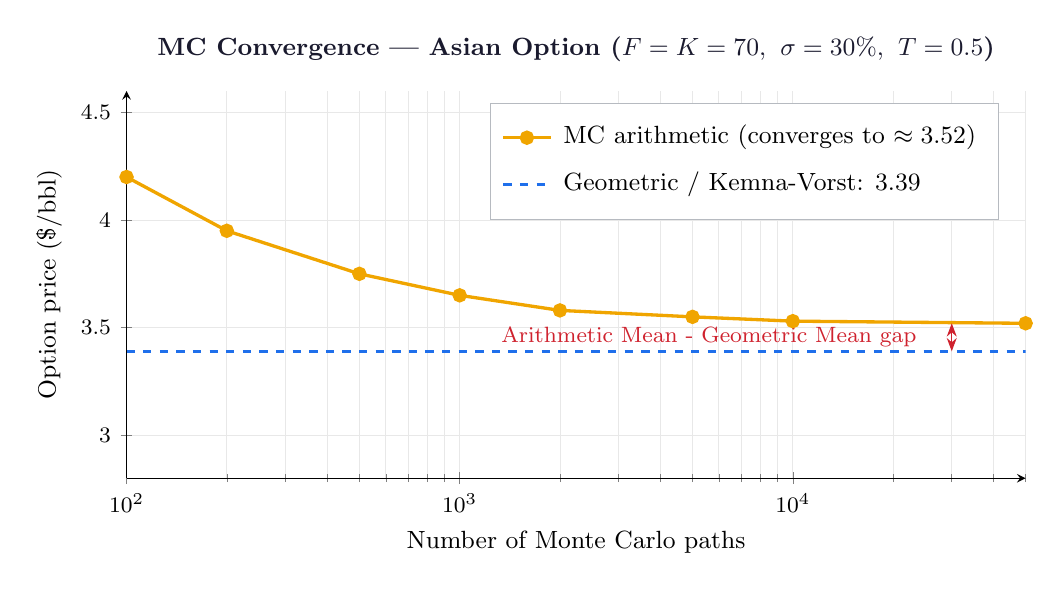
\begin{tikzpicture}
\begin{axis}[width=13cm,height=6.5cm,
  xlabel={Number of Monte Carlo paths},ylabel={Option price (\$/bbl)},
  xmode=log,xmin=100,xmax=50000,ymin=2.8,ymax=4.6,
  grid=both,axis lines=left,
  title={MC Convergence --- Asian Option ($F=K=70,\ \sigma=30\%,\ T=0.5$)},
  legend style={at={(0.97,0.97)},anchor=north east}]
\addplot[color=amber,very thick,mark=*,mark size=2pt] coordinates
  {(100,4.20)(200,3.95)(500,3.75)(1000,3.65)
   (2000,3.58)(5000,3.55)(10000,3.53)(50000,3.52)};
\addlegendentry{MC arithmetic (converges to $\approx 3.52$)}
\addplot[color=accentblue,very thick,dashed,domain=100:50000]{3.39};
\addlegendentry{Geometric / Kemna-Vorst: $3.39$}
\draw[{Stealth}-{Stealth},thin,color=signalred]
  (axis cs:30000,3.39)--(axis cs:30000,3.52);
\node[font=\footnotesize,color=signalred]at(axis cs:5600,3.455){ Arithmetic Mean - Geometric Mean gap};
\end{axis}
\end{tikzpicture}
\end{center}

\begin{notebox}
\textbf{AM-GM ordering:} The arithmetic average $\geq$ geometric average (AM-GM inequality). Therefore the MC arithmetic price is always $\geq$ the analytical Kemna-Vorst price. OCDAP verifies this automatically as a numerical sanity check.
\end{notebox}

\subsection{Geometric Average --- Kemna-Vorst (1990)}

\begin{equation}
\sigma_g=\sigma\sqrt{\frac{2N+1}{6(N+1)}},\qquad
b_g=\frac12\!\left(-\frac{\sigma^2}{6}+\sigma_g^2\right),\qquad
F_g=F\cdot e^{b_g T}
\end{equation}

The geometric Asian is then priced as a Black-76 option with parameters
$(\sigma_g,\,F_g)$.

%==============================================================================
\section{Crack Spread Option Pricer}
%==============================================================================

\subsection{The Refining Margin}

A refiner is \textbf{naturally long the crack spread}: it buys crude oil ($F_1$)
and sells refined products ($F_2$, $F_3$). It hedges by buying a \textbf{put on
the crack spread} --- protecting against margin compression.

\medskip
\begin{center}
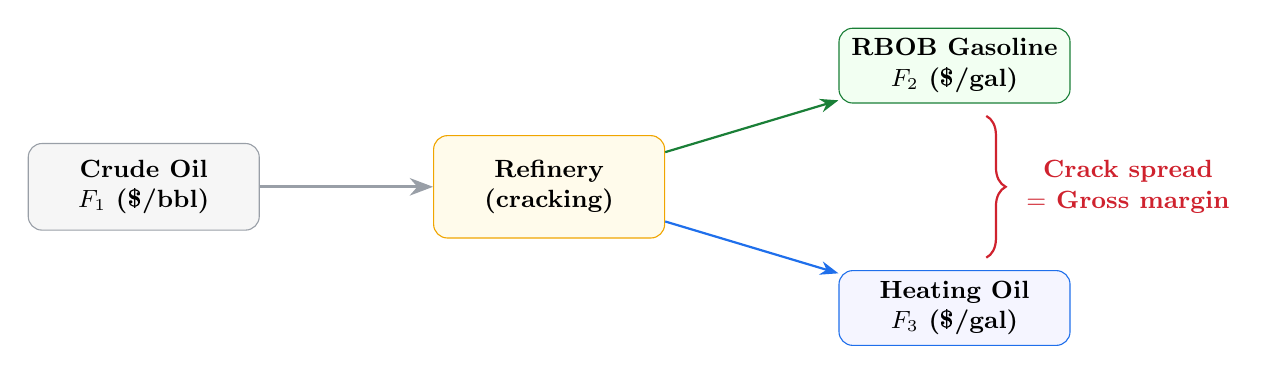
\begin{tikzpicture}[node distance=2.2cm]
\node[draw=signalgray!70,fill=gray!7,rounded corners=5pt,
      text width=2.7cm,minimum height=1.1cm,
      font=\small\bfseries,align=center](crude)
  {Crude Oil\\$F_1$ (\$/bbl)};
\node[draw=amber,fill=notebg,rounded corners=5pt,
      text width=2.7cm,minimum height=1.3cm,
      font=\small\bfseries,align=center,right=of crude](ref)
  {Refinery\\(cracking)};
\node[draw=signalgreen,fill=green!5,rounded corners=5pt,
      text width=2.7cm,minimum height=0.95cm,
      font=\small\bfseries,align=center,
      above right=0.4cm and 2.2cm of ref](rbob)
  {RBOB Gasoline\\$F_2$ (\$/gal)};
\node[draw=accentblue,fill=blue!4,rounded corners=5pt,
      text width=2.7cm,minimum height=0.95cm,
      font=\small\bfseries,align=center,
      below right=0.4cm and 2.2cm of ref](ho)
  {Heating Oil\\$F_3$ (\$/gal)};
\draw[-{Stealth},very thick,color=signalgray!70](crude)--(ref);
\draw[-{Stealth},thick,color=signalgreen](ref)--(rbob);
\draw[-{Stealth},thick,color=accentblue](ref)--(ho);
\draw[decorate,decoration={brace,amplitude=7pt},
      color=signalred,thick](10.7,0.9)--(10.7,-0.9);
\node[font=\small\bfseries,color=signalred,align=center]
  at(12.5,0){\shortstack{Crack spread\\$=$ Gross margin}};
\end{tikzpicture}
\end{center}

\medskip
The most common crack spread configurations:

\begin{center}
\renewcommand{\arraystretch}{1.6}
\begin{tabularx}{\textwidth}{>{\bfseries}l X r}
\toprule
Name & Formula & Typical value \\
\midrule
3-2-1 crack &
  $\tfrac{1}{3}(2\cdot F_\text{RBOB}\cdot42 + F_\text{HO}\cdot42) - F_\text{WTI}$ &
  \$12--20/bbl \\
Simple crack &
  $F_\text{RBOB}\cdot42 - F_\text{WTI}$ &
  \$10--16/bbl \\
Jet crack &
  $F_\text{Jet CIF NWE} - F_\text{Brent}$ &
  \$70--100/mt \\
Spark spread &
  $F_\text{power} - \text{HR}\times F_\text{gas}$ &
  \$3--8/MWh \\
\bottomrule
\end{tabularx}
\end{center}

\subsection{Kirk (1995) Approximation}

\begin{equation}
\alpha=\frac{F_2}{F_2+Ke^{-rT}},\qquad
\boxed{\sigma_\text{Kirk}=\sqrt{\sigma_1^2+(\alpha\sigma_2)^2
-2\rho\,\sigma_1\sigma_2\,\alpha}}
\end{equation}

\begin{keybox}{Why Kirk and not Margrabe?}
Margrabe's exact formula only prices exchange options with $K=0$.
Crack spread options always have $K>0$ (the target margin). Kirk (1995)
extends Margrabe to non-zero strikes and is the industry standard.
Accuracy is excellent for $\rho>0.70$, which always holds for crude vs
refined products (typical $\rho\approx0.85$--$0.95$).
\end{keybox}

\begin{center}
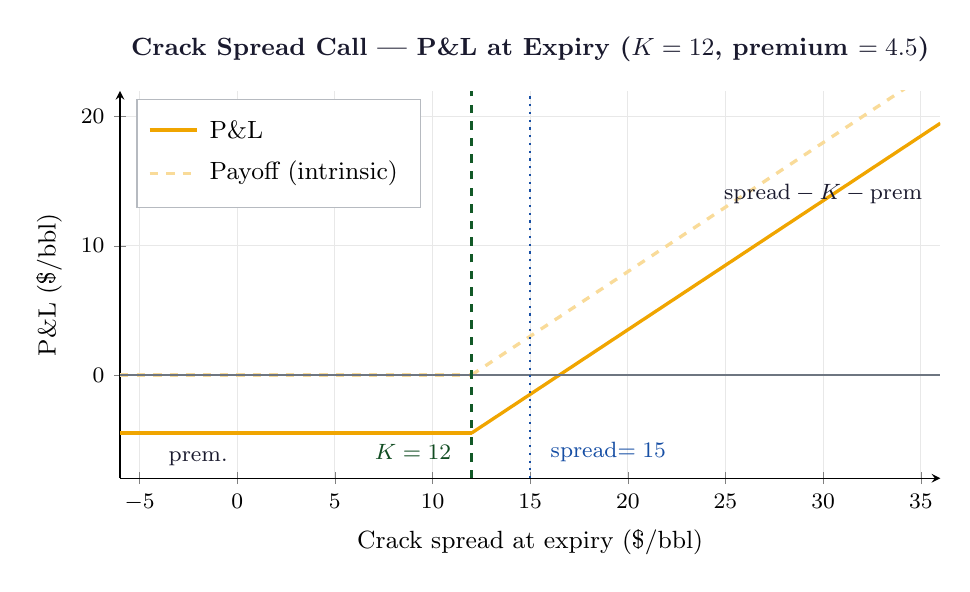
\begin{tikzpicture}
\begin{axis}[width=12cm,height=6.5cm,
  xlabel={Crack spread at expiry (\$/bbl)},ylabel={P\&L (\$/bbl)},
  xmin=-6,xmax=36,ymin=-8,ymax=22,
  grid=both,axis lines=left,
  title={Crack Spread Call --- P\&L at Expiry ($K=12$, premium $=4.5$)},
  legend style={at={(0.02,0.98)},anchor=north west}]
\addplot[color=amber,very thick,domain=-6:12]{-4.5};
\addplot[color=amber!40,very thick,dashed,domain=-6:12]{0};
\addplot[color=amber!40,very thick,dashed,domain=12:36]{x-12};
\addplot[color=amber,very thick,domain=12:36]{x-16.5};
\addplot[color=signalgray,thin,domain=-6:36]{0};
\draw[dashed,color=signalgreen!70!black,thick]
  (axis cs:12,-8)--(axis cs:12,22);
\draw[dotted,color=accentblue!70!black,thick]
  (axis cs:15,-8)--(axis cs:15,22);
\addlegendentry{P\&L}
\addlegendentry{Payoff (intrinsic)}
\node[font=\footnotesize,color=signalgreen!60!black]at(axis cs:9,-6){$K=12$};
\node[font=\footnotesize,color=accentblue!70!black]at(axis cs:19,-6){spread$=15$};
\node[font=\footnotesize,color=darktext]at(axis cs:-2,-6.5){prem.};
\node[font=\footnotesize,color=darktext]at(axis cs:30,14){$\text{spread}-K-\text{prem}$};
\end{axis}
\end{tikzpicture}
\end{center}

%==============================================================================
\section{Calendar Spread Option Pricer}
%==============================================================================

\subsection{What a Calendar Spread Option Trades}

A calendar spread option gives exposure to the \textbf{slope of the forward
curve}: the difference between two delivery dates on the same commodity.

\begin{itemize}[itemsep=3pt]
\item \textbf{Call on M1-M6 spread}: pays off when backwardation widens
      (M1 rises relative to M6). Used by traders who believe near-term
      supply will tighten further.
\item \textbf{Put on M1-M6 spread}: pays off when contango deepens.
      Used by storage players who want to hedge their carry trade.
\end{itemize}

\begin{center}
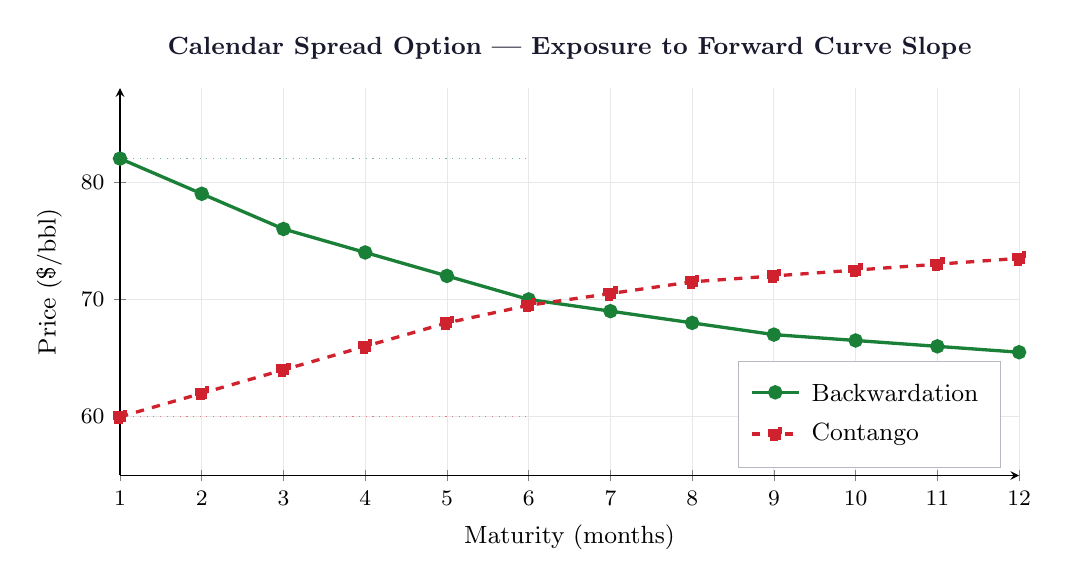
\begin{tikzpicture}
\begin{axis}[width=13cm,height=6.5cm,
  xlabel={Maturity (months)},ylabel={Price (\$/bbl)},
  xmin=1,xmax=12,ymin=55,ymax=88,
  xtick={1,2,3,4,5,6,7,8,9,10,11,12},
  grid=both,axis lines=left,
  title={Calendar Spread Option --- Exposure to Forward Curve Slope},
  legend style={at={(0.98,0.02)},anchor=south east}]
\addplot[color=signalgreen,very thick,mark=*,mark size=2pt] coordinates
  {(1,82)(2,79)(3,76)(4,74)(5,72)(6,70)
   (7,69)(8,68)(9,67)(10,66.5)(11,66)(12,65.5)};
\addlegendentry{Backwardation}
\addplot[color=signalred,very thick,mark=square*,mark size=2pt,dashed] coordinates
  {(1,60)(2,62)(3,64)(4,66)(5,68)(6,69.5)
   (7,70.5)(8,71.5)(9,72)(10,72.5)(11,73)(12,73.5)};
\addlegendentry{Contango}
\draw[{Stealth}-{Stealth},very thick,color=darktext]
  (axis cs:0.55,82)--(axis cs:0.55,60);
\node[font=\footnotesize,color=darktext,rotate=90,anchor=south]
  at(axis cs:0.72,71){\shortstack{M1-M6\\spread}};
\draw[dotted,thin,color=signalgreen!60](axis cs:1,82)--(axis cs:6,82);
\draw[dotted,thin,color=signalred!60](axis cs:1,60)--(axis cs:6,60);
\end{axis}
\end{tikzpicture}
\end{center}

\subsection{Kirk on the Term Structure}

\begin{equation}
\alpha=\frac{F_\text{near}}{F_\text{near}+Ke^{-rT}},\qquad
\sigma_\text{Kirk}=\sqrt{\sigma_\text{far}^2
+(\alpha\,\sigma_\text{near})^2-2\rho\,\sigma_\text{far}\,\sigma_\text{near}\,\alpha}
\end{equation}

OCDAP defaults to $\sigma_\text{near}=1.05\,\sigma$ and
$\sigma_\text{far}=0.90\,\sigma$, reflecting the empirical observation that
short-dated contracts are more volatile than deferred contracts.

%==============================================================================
\section{Commodity Swap Pricer}
%==============================================================================

\subsection{What is a Commodity Swap?}

A commodity swap is a bilateral contract in which one party pays a
\textbf{fixed price} $K$ per period and receives the \textbf{floating market
price} $F_i$.

\begin{center}
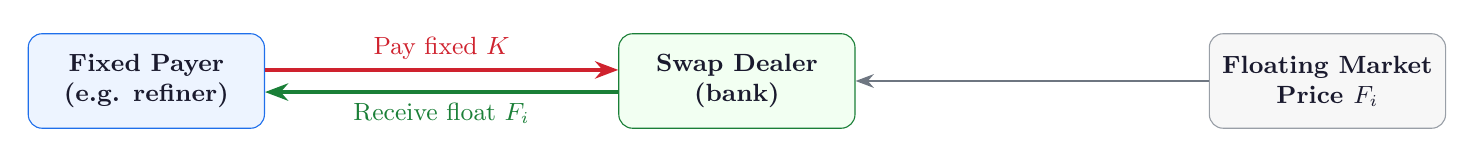
\begin{tikzpicture}
\node[draw=accentblue,fill=boxbg,rounded corners=5pt,
      minimum width=3.0cm,minimum height=1.2cm,
      font=\small\bfseries,align=center,text=darktext](buyer)
  at(0,0){Fixed Payer\\(e.g. refiner)};
\node[draw=signalgreen,fill=green!5,rounded corners=5pt,
      minimum width=3.0cm,minimum height=1.2cm,
      font=\small\bfseries,align=center,text=darktext](dealer)
  at(7.5,0){Swap Dealer\\(bank)};
\node[draw=signalgray!70,fill=gray!6,rounded corners=5pt,
      minimum width=3.0cm,minimum height=1.2cm,
      font=\small\bfseries,align=center,text=darktext](mkt)
  at(15,0){Floating Market\\Price $F_i$};
\draw[-{Stealth},very thick,color=signalred]
  ([yshift=4pt]buyer.east) -- 
  node[above,font=\small,color=signalred]{Pay fixed $K$}
  ([yshift=4pt]dealer.west);
\draw[-{Stealth},very thick,color=signalgreen]
  ([yshift=-4pt]dealer.west) -- 
  node[below,font=\small,color=signalgreen]{Receive float $F_i$}
  ([yshift=-4pt]buyer.east);
\draw[-{Stealth},thick,color=signalgray](mkt.west)--(dealer.east);
\end{tikzpicture}
\end{center}

\subsection{Cash Flow Diagram}
\begin{center}
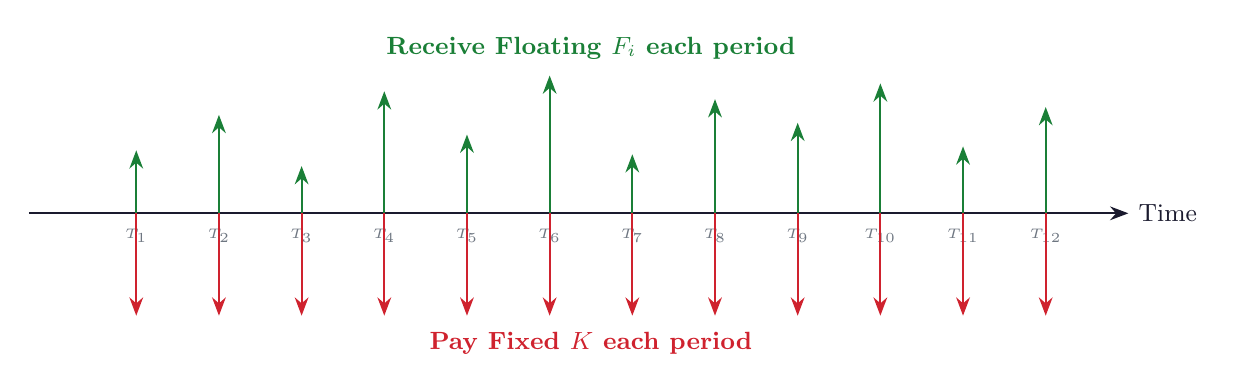
\begin{tikzpicture}[xscale=1.05]
\draw[-{Stealth},thick,color=darktext](-0.3,0)--(13.0,0)
  node[right,font=\small]{Time};
\foreach \t in {1,...,12}{
  \draw[thin,color=signalgray](\t,-0.1)--(\t,0.1);
  \node[font=\tiny,color=signalgray]at(\t,-0.28){$T_{\t}$};}
\foreach \t in {1,...,12}
  \draw[-{Stealth},thick,color=signalred](\t,0)--(\t,-1.3);
\node[font=\small\bfseries,color=signalred]at(6.5,-1.65){Pay Fixed $K$ each period};
\foreach \t/\h in {1/.8,2/1.25,3/.6,4/1.55,5/1.0,6/1.75,
                   7/.75,8/1.45,9/1.15,10/1.65,11/.85,12/1.35}
  \draw[-{Stealth},thick,color=signalgreen](\t,0)--(\t,\h);
\node[font=\small\bfseries,color=signalgreen]at(6.5,2.1){Receive Floating $F_i$ each period};
\end{tikzpicture}
\end{center}

\begin{equation}
\boxed{\mathrm{NPV}=\sum_{i=1}^{N}e^{-rT_i}(F_i-K)\cdot\mathrm{notional}}
\qquad
K^*=\frac{\sum_{i=1}^{N}e^{-rT_i}F_i}{\sum_{i=1}^{N}e^{-rT_i}}
\end{equation}

$K^*$ is the \textbf{fair fixed rate}: the level at which NPV $= 0$ at inception. It is the present-value-weighted average of all forward prices.

\subsection{DV01 and Sensitivity}

\begin{center}
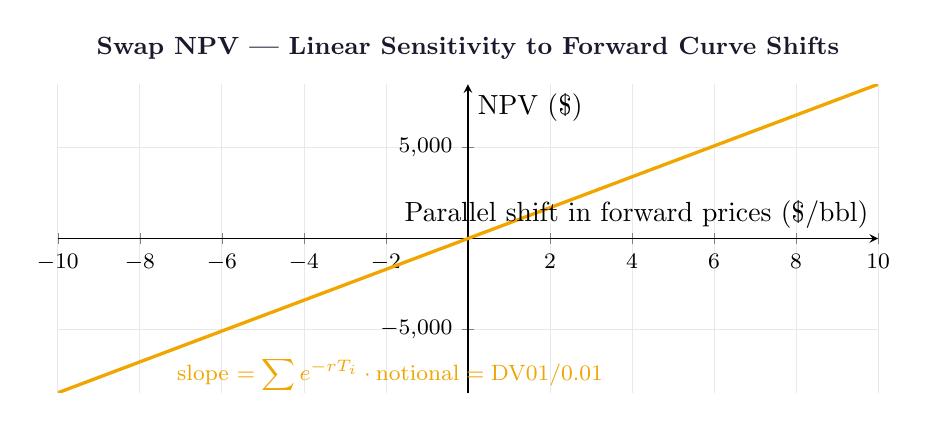
\begin{tikzpicture}
\begin{axis}[width=12cm,height=5.5cm,
  xlabel={Parallel shift in forward prices (\$/bbl)},
  ylabel={NPV (\$)},
  xmin=-10,xmax=10,
  grid=both,axis lines=center,
  title={Swap NPV --- Linear Sensitivity to Forward Curve Shifts}]
\addplot[color=amber,very thick,domain=-10:10]{x*850};
\node[font=\footnotesize,color=amber]at(axis cs:-1.9,-8000)
  {slope $=\displaystyle\sum_i e^{-rT_i}\cdot\text{notional}=\text{DV01}/0.01$};
\end{axis}
\end{tikzpicture}
\end{center}

\textbf{DV01} (Dollar Value of 1 basis point) measures the change in NPV for a 0.01\% parallel shift in all forward prices --- the primary sensitivity metric for swap portfolios.

%==============================================================================
\section{Barrier Option Pricer}
%==============================================================================

\subsection{Types of Barrier Options}

A barrier option activates (knock-in) or terminates (knock-out) if the underlying touches a barrier level $B$ during the option's life.

\begin{center}
\renewcommand{\arraystretch}{1.6}
\begin{tabularx}{\textwidth}{>{\bfseries}l l X l}
\toprule
Type & Barrier & Payoff condition & Primary use \\
\midrule
Down-and-Out (KO) & $B<S$ & Vanilla payoff if $\min_t S_t > B$ & Most common in energy \\
Down-and-In  (KI) & $B<S$ & Vanilla payoff only if $\min_t S_t \leq B$ & Speculative \\
Up-and-Out   (KO) & $B>S$ & Vanilla payoff if $\max_t S_t < B$ & Producer hedge \\
Up-and-In    (KI) & $B>S$ & Vanilla payoff only if $\max_t S_t \geq B$ & Structured products \\
\bottomrule
\end{tabularx}
\end{center}

\textbf{Why Down-and-Out Call is most common in energy:}
A consumer buys a call to hedge against rising prices. Adding a down barrier
makes the option cheaper --- if the price collapses below $B$, the option is
knocked out, but the consumer doesn't need protection anyway because the
market is giving them a cheap purchase price.

\subsection{Daily Monte Carlo Simulation}

Analytical barrier formulas assume a continuous barrier. In practice, barriers
are monitored \textbf{daily} (at settlement), so daily-step MC is the correct method:

\begin{equation}
C_\text{KO}=e^{-rT}\cdot\mathbb{E}\Big[
\max(S_T-K,\,0)\cdot\mathbf{1}_{\{\min_{0\leq t\leq T}S_t>B\}}\Big]
\end{equation}

\begin{center}
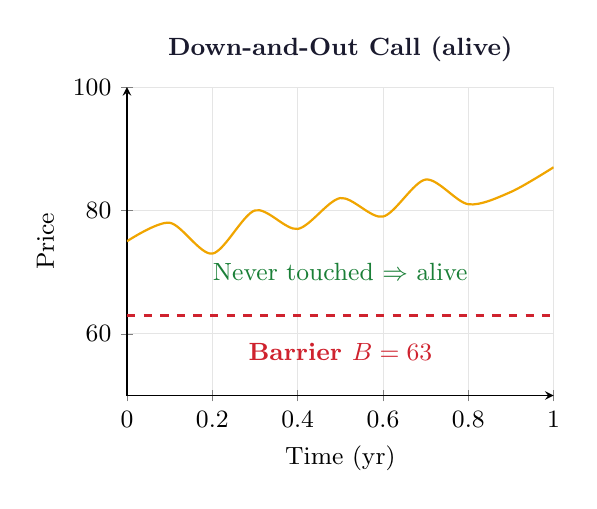
\begin{tikzpicture}
\begin{axis}[
    width=7cm,height=5.5cm,
    xlabel={Time (yr)},ylabel={Price},
    xmin=0,xmax=1,ymin=50,ymax=100,
    grid=both,grid style={draw=gray!20},
    axis lines=left,
    tick label style={font=\small},
    label style={font=\small},
    title={\small\bfseries Down-and-Out Call (alive)},
    title style={color=darktext}
]
\addplot[color=amber,thick,smooth] coordinates
  {(0,75)(0.1,78)(0.2,73)(0.3,80)(0.4,77)(0.5,82)(0.6,79)(0.7,85)(0.8,81)(0.9,83)(1.0,87)};
\addplot[very thick,dashed,color=signalred,domain=0:1] {63};
\node[color=signalred,font=\small\bfseries] at (axis cs:0.5,57) {Barrier $B=63$};
\node[color=signalgreen,font=\small] at (axis cs:0.5,70) {Never touched $\Rightarrow$ alive};
\end{axis}
\end{tikzpicture}
\hspace{0.5cm}
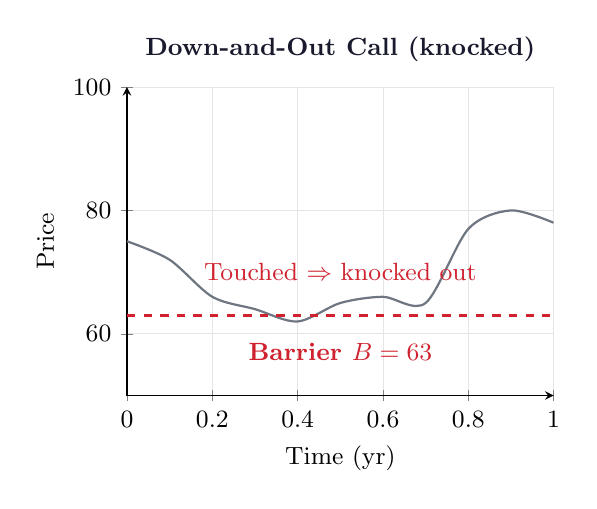
\begin{tikzpicture}
\begin{axis}[
    width=7cm,height=5.5cm,
    xlabel={Time (yr)},ylabel={Price},
    xmin=0,xmax=1,ymin=50,ymax=100,
    grid=both,grid style={draw=gray!20},
    axis lines=left,
    tick label style={font=\small},
    label style={font=\small},
    title={\small\bfseries Down-and-Out Call (knocked)},
    title style={color=darktext}
]
\addplot[color=signalgray,thick,smooth] coordinates
  {(0,75)(0.1,72)(0.2,66)(0.3,64)(0.4,62)(0.5,65)(0.6,66)(0.7,65)(0.8,77)(0.9,80)(1.0,78)};
\addplot[very thick,dashed,color=signalred,domain=0:1] {63};
\node[color=signalred,font=\small\bfseries] at (axis cs:0.5,57) {Barrier $B=63$};
\node[color=signalred,font=\small] at (axis cs:0.5,70) {Touched $\Rightarrow$ knocked out};
\end{axis}
\end{tikzpicture}
\end{center}


\subsection{Price vs Barrier Level}

\begin{center}
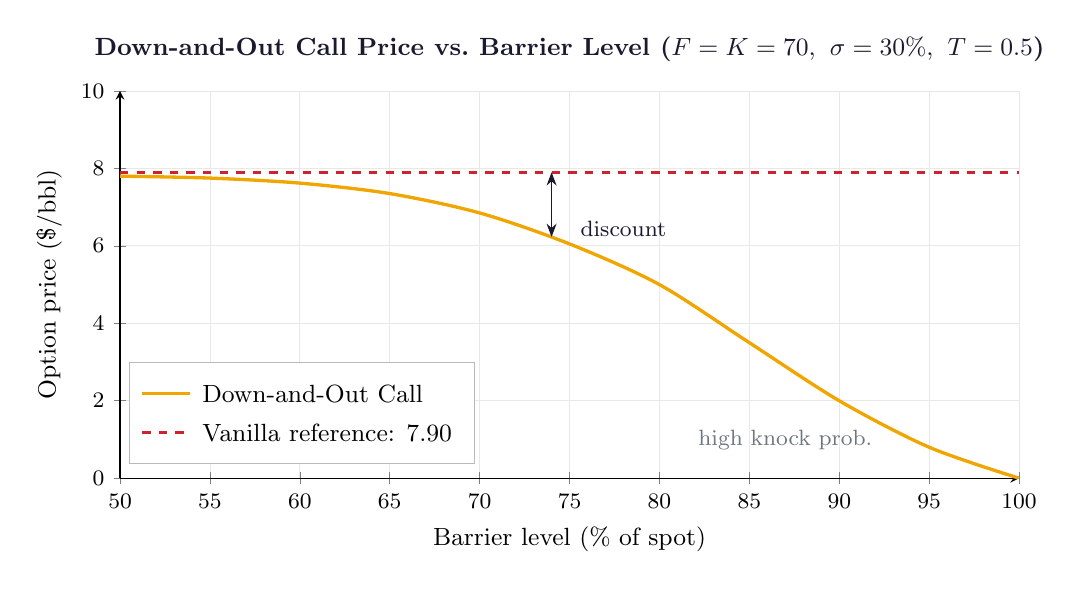
\begin{tikzpicture}
\begin{axis}[width=13cm,height=6.5cm,
  xlabel={Barrier level (\% of spot)},ylabel={Option price (\$/bbl)},
  xmin=50,xmax=100,ymin=0,ymax=10,
  grid=both,axis lines=left,
  title={Down-and-Out Call Price vs.\ Barrier Level
         ($F=K=70,\ \sigma=30\%,\ T=0.5$)},
  legend style={at={(0.01,0.3)},anchor=north west}]
\addplot[color=amber,very thick,smooth] coordinates
  {(50,7.80)(55,7.75)(60,7.62)(65,7.35)
   (70,6.85)(75,6.05)(80,5.00)(85,3.50)(90,2.00)(95,0.80)(100,0)};
\addlegendentry{Down-and-Out Call}
\addplot[color=signalred,very thick,dashed,domain=50:100]{7.90};
\addlegendentry{Vanilla reference: $7.90$}
\draw[{Stealth}-{Stealth},thin,color=darktext]
  (axis cs:74,6.23)--(axis cs:74,7.90);
\node[font=\footnotesize,color=darktext]at(axis cs:78,6.45){discount};
\node[font=\footnotesize,color=signalgray]at(axis cs:87,1.0){high knock prob.};
\end{axis}
\end{tikzpicture}
\end{center}

As the barrier moves closer to the spot ($B\to S$), the knock-out probability
increases and the barrier price converges to zero. At $B=0$, the barrier option
equals the vanilla. The \textbf{discount} vs vanilla is the price the buyer pays
for the knock-out risk.

%==============================================================================
\section{Volatility Surface}
%==============================================================================

\subsection{The Smile and Skew}

In real commodity markets, implied volatility is not flat across strikes.
Two empirical patterns emerge:

\begin{itemize}[itemsep=3pt]
\item \textbf{Skew} ($\partial\sigma/\partial K < 0$): OTM puts more expensive
      than OTM calls. Reflects fear of sharp downside moves (supply shocks,
      demand collapse, geopolitical events).
\item \textbf{Smile} (curvature): both wings more expensive than ATM. Reflects
      fat tails in the price distribution --- extreme moves in both directions
      are priced in.
\end{itemize}

\begin{center}
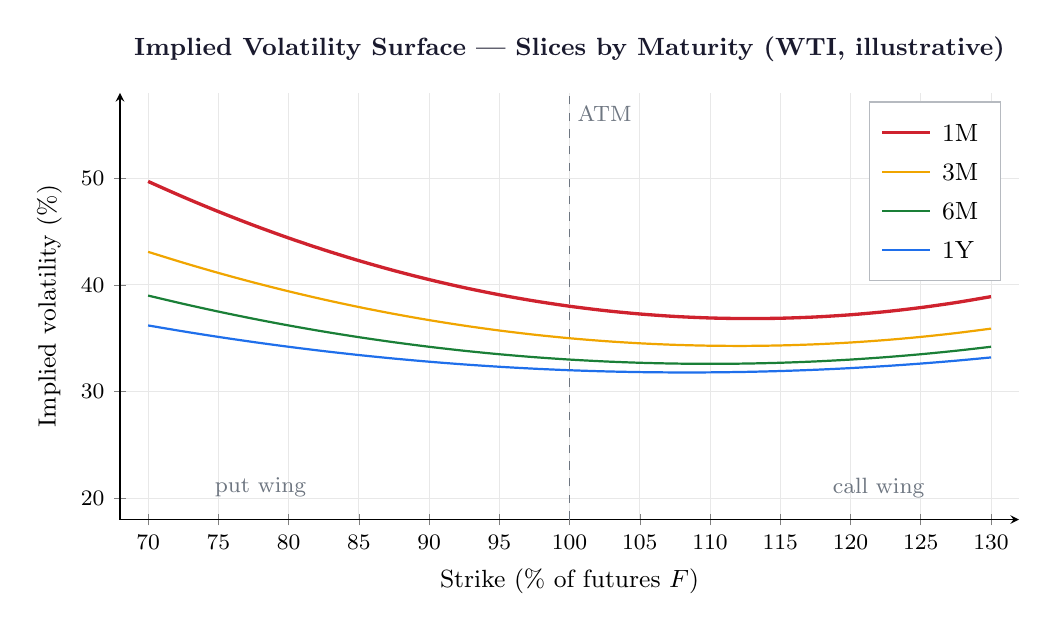
\begin{tikzpicture}
\begin{axis}[width=13cm,height=7cm,
  xlabel={Strike (\% of futures $F$)},ylabel={Implied volatility (\%)},
  xmin=68,xmax=132,ymin=18,ymax=58,
  grid=both,axis lines=left,
  title={Implied Volatility Surface --- Slices by Maturity (WTI, illustrative)},
  legend style={at={(0.98,0.98)},anchor=north east}]
\addplot[color=signalred,very thick,smooth,domain=70:130]
  {38-0.18*(x-100)+0.007*(x-100)^2};
\addlegendentry{1M}
\addplot[color=amber,thick,smooth,domain=70:130]
  {35-0.12*(x-100)+0.005*(x-100)^2};
\addlegendentry{3M}
\addplot[color=signalgreen,thick,smooth,domain=70:130]
  {33-0.08*(x-100)+0.004*(x-100)^2};
\addlegendentry{6M}
\addplot[color=accentblue,thick,smooth,domain=70:130]
  {32-0.05*(x-100)+0.003*(x-100)^2};
\addlegendentry{1Y}
\draw[dashed,color=signalgray,thin](axis cs:100,18)--(axis cs:100,58);
\node[font=\footnotesize,color=signalgray]at(axis cs:102.5,56){ATM};
\node[font=\footnotesize,color=signalgray]at(axis cs:78,21){put wing};
\node[font=\footnotesize,color=signalgray]at(axis cs:122,21){call wing};
\end{axis}
\end{tikzpicture}
\end{center}

\subsection{Parametric Model}

\begin{equation}
\sigma(K,T)=
\underbrace{\sigma_\text{ATM}(1+\nu\sqrt{T})}_{\text{term structure}}
+\underbrace{\text{skew}\cdot\ln\tfrac{K}{F}}_{\text{slope}}
+\underbrace{\text{curvature}\cdot\!\Bigl(\ln\tfrac{K}{F}\Bigr)^2}_{\text{wings}}
\end{equation}

\begin{center}
\begin{tabularx}{\textwidth}{>{\bfseries}l X r}
\toprule
Parameter & Economic meaning & WTI typical \\
\midrule
ATM vol $\sigma$ &
  Base implied vol at the money. Higher for nat gas ($\sim55\%$),
  lower for gold ($\sim15\%$). & 30\% \\
Skew &
  Negative in most commodity markets. Reflects downside fear.
  More negative for crude than for gold. & $-0.03$ \\
Curvature &
  Symmetric wing steepness. Positive values create a U-shaped smile. & $+0.05$ \\
Steepness $\nu$ &
  Term structure slope. Short-dated vol $>$ long-dated vol
  due to mean-reversion of commodity prices. & $+0.08$ \\
\bottomrule
\end{tabularx}
\end{center}

%==============================================================================
\section{Forward Curve Data Layer}
%==============================================================================

\subsection{Cost-of-Carry Model}

When live data is unavailable, OCDAP generates a synthetic fallback curve:

\begin{equation}
F(T)=S\cdot e^{(r+u-cy)\,T}
\end{equation}

where $u$ is the annualised storage cost and $cy$ the convenience yield.

\begin{itemize}[itemsep=3pt]
\item $cy > r+u$: \textbf{backwardation} --- physical scarcity premium
\item $cy < r+u$: \textbf{contango} --- storage surplus, carry dominates
\item $cy = r+u$: flat curve at fair value
\end{itemize}

\begin{center}
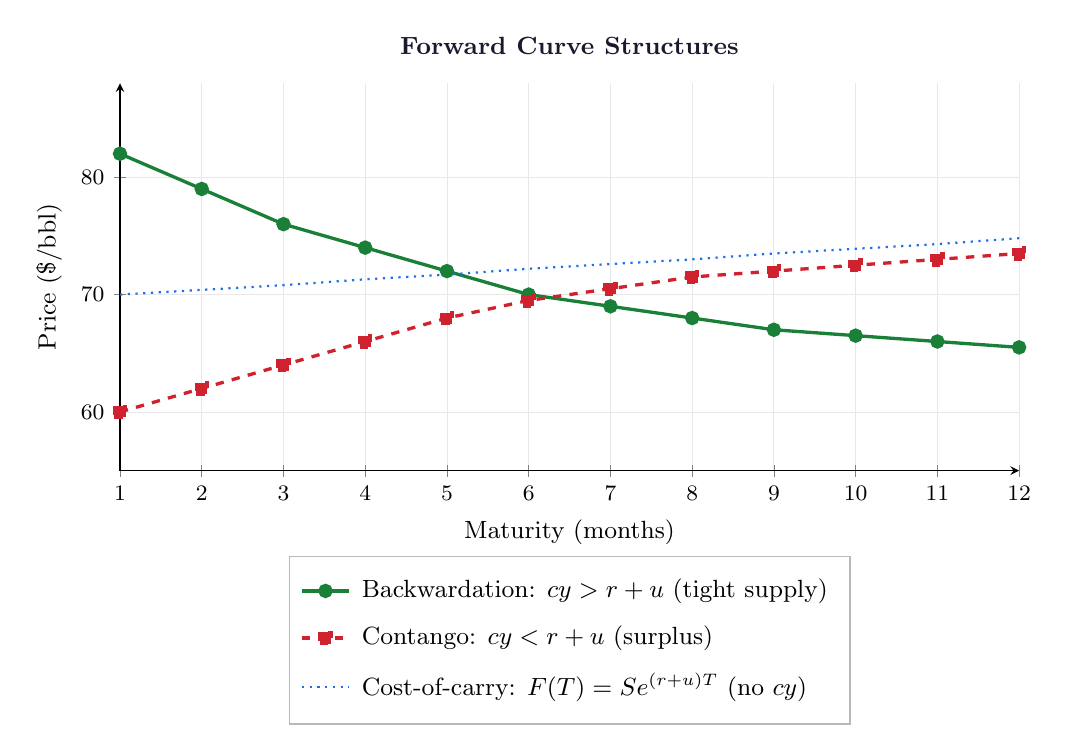
\begin{tikzpicture}
\begin{axis}[width=13cm,height=6.5cm,
  xlabel={Maturity (months)},ylabel={Price (\$/bbl)},
  xmin=1,xmax=12,ymin=55,ymax=88,
  xtick={1,2,3,4,5,6,7,8,9,10,11,12},
  grid=both,axis lines=left,
  title={Forward Curve Structures},
  legend style={at={(0.5,-0.22)},anchor=north,font=\small}]
\addplot[color=signalgreen,very thick,mark=*,mark size=2pt] coordinates
  {(1,82)(2,79)(3,76)(4,74)(5,72)(6,70)
   (7,69)(8,68)(9,67)(10,66.5)(11,66)(12,65.5)};
\addlegendentry{Backwardation: $cy>r+u$ (tight supply)}
\addplot[color=signalred,very thick,mark=square*,mark size=2pt,dashed] coordinates
  {(1,60)(2,62)(3,64)(4,66)(5,68)(6,69.5)
   (7,70.5)(8,71.5)(9,72)(10,72.5)(11,73)(12,73.5)};
\addlegendentry{Contango: $cy<r+u$ (surplus)}
\addplot[color=accentblue,thick,dotted] coordinates
  {(1,70)(2,70.4)(3,70.8)(4,71.3)(5,71.7)(6,72.2)
   (7,72.6)(8,73)(9,73.5)(10,73.9)(11,74.3)(12,74.8)};
\addlegendentry{Cost-of-carry: $F(T)=Se^{(r+u)T}$ (no $cy$)}
\end{axis}
\end{tikzpicture}
\end{center}

\subsection{Data Sources and Commodity Registry}

\begin{center}
\renewcommand{\arraystretch}{1.5}
\begin{tabularx}{\textwidth}{>{\bfseries}l c c X}
\toprule
Family & Count & Source & Examples \\
\midrule
Energy              & 7  & Yahoo Finance  & WTI, Brent, Nat Gas, RBOB, Gasoil \\
Metals              & 5  & Yahoo Finance  & Gold, Silver, Copper, Platinum, Palladium \\
Agriculture         & 15 & Yahoo Finance  & Corn, Wheat, Soybeans, Sugar, Coffee, Cattle \\
Base Metals (LME)   & 9  & TradingView    & Copper, Aluminum, Zinc, Nickel, Lead \\
Energy (additional) & 8  & TradingView    & TTF, NBP, Coal API2/4, Uranium, Carbon EUA \\
Freight             & 4  & TradingView    & Capesize, Panamax, Supramax, VLCC \\
Carbon              & 4  & TradingView    & EU EUA, UK UKA, California CCA, RGGI \\
\midrule
\textbf{Total} & \textbf{65+} & & \\
\bottomrule
\end{tabularx}
\end{center}

%==============================================================================
\section{Applications and Extensions}
%==============================================================================

\subsection{Typical Users}

\begin{center}
\renewcommand{\arraystretch}{1.8}
\begin{tabularx}{\textwidth}{>{\bfseries}l X}
\toprule
User & How OCDAP helps \\
\midrule
Options Desk &
  Price vanilla and barrier options on any of 65+ commodities.
  Read off full Greeks for hedging. Assess the vol surface to identify
  whether implied vol is rich or cheap relative to ATM. \\
Physical Hedger &
  Price Asian calls based on monthly average procurement costs.
  Lock in a fixed price for 12+ months with a commodity swap.
  Compare vanilla vs barrier premium to find the optimal hedge structure. \\
Margin Hedger &
  Price 3-2-1, jet crack and spark spread options to protect gross
  refining or generation margins. Compute break-even spread levels. \\
Spread Trader &
  Price calendar spread options to speculate on steepening or flattening.
  Trade the roll yield in backwardation markets. \\
\bottomrule
\end{tabularx}
\end{center}

\subsection{Possible Quantitative Extensions}

\textbf{Implied vol from real option chains.}
Yahoo Finance exposes option chain data for WTI, Gold and Corn via
\texttt{yfinance}. OCDAP could extract market-implied vols per strike and
maturity to overlay against the parametric model.

\textbf{SABR stochastic volatility.}
The SABR model is the industry standard for capturing the vol smile in
commodity and interest rate derivatives. It produces more realistic OTM prices
and is consistent with the market's implied vol surface.

\textbf{Swing options.}
Standard in European gas and power markets (Engie, TotalEnergies, EDF).
The holder has the right to take or deliver gas at a variable daily volume
within contractual bounds. Pricing requires dynamic programming.

\textbf{Schwartz-Smith Monte Carlo.}
Using calibrated SS parameters $(\kappa,\xi_0,\sigma_\chi,\sigma_\xi)$ as
diffusion inputs to price path-dependent exotics in a single consistent framework.

%==============================================================================
\section{Conclusion}
%==============================================================================

OCDAP demonstrates how a professional-grade commodity derivatives pricer can
be built entirely in Python with freely available market data.

Six pricing engines cover the full spectrum of products used by commodity
desks: vanilla options (Black-76), average-price options (Monte Carlo), spread
options (Kirk 1995), curve slope options, fixed-for-floating swaps, and
path-dependent barrier options. The expiry-aware ticker logic ensures prices
always come from live, non-expired contracts.

Together with CFCAP, OCDAP provides a complete analytical stack: forward curve
analysis and trading signals on one side, derivatives pricing and risk on the other.

\vspace{1.2cm}
\begin{center}
\textit{Built with Python\,$\cdot$\,Yahoo Finance\,$\cdot$\,TradingView}
\end{center}

\end{document}
